\documentclass[border=10pt]{standalone} 
\usepackage{tikz}

\usetikzlibrary{calc}
\usetikzlibrary{arrows}
\usetikzlibrary{shadows}
\usetikzlibrary{patterns}
\usetikzlibrary{positioning}
\usetikzlibrary{shapes}
\usetikzlibrary{3d}
%\usetikzlibrary{automata}
\usetikzlibrary{fit}

\tikzset{block/.style={draw, text centered, fill=gray!10,drop shadow}}
\tikzset{connect/.style={draw, line width=1 pt}}

\begin{document}


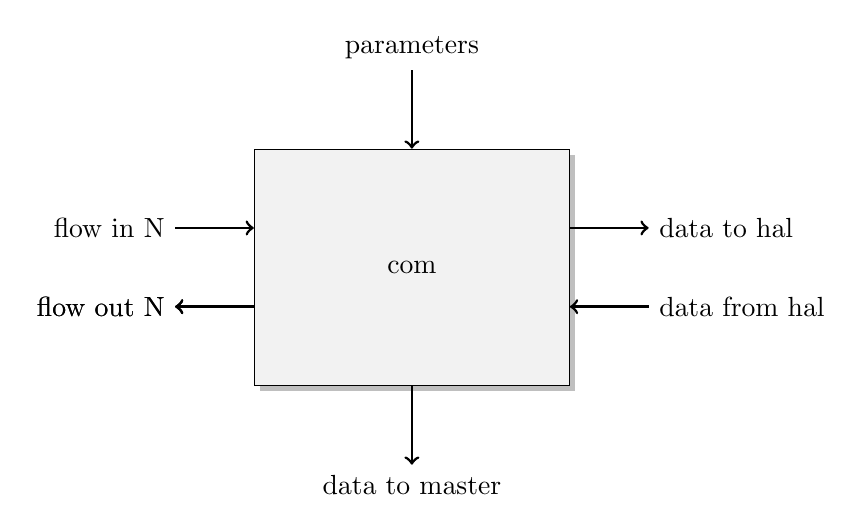
\begin{tikzpicture}

\node[block,minimum height=3cm,minimum width=4cm] (com) {com};

\path[connect,<-] (com.north) -- ++ (0,1cm) node[above]{parameters};
\path[connect,<-] ([yshift=0.5cm]com.west) -- ++ (-1cm,0cm) node[left]{flow in N};
\path[connect,->] ([yshift=-0.5cm]com.west) -- ++ (-1cm,0cm) node[left]{flow out N};
\path[connect,->] ([yshift=-0.5cm]com.west) -- ++ (-1cm,0cm) node[left]{flow out N};
\path[connect,->] ([yshift=0.5cm]com.east) -- ++ (1cm,0cm) node[right]{data to hal};
\path[connect,<-] ([yshift=-0.5cm]com.east) -- ++ (1cm,0cm) node[right]{data from hal};
\path[connect,->] (com.south) -- ++ (0cm,-1cm) node[below]{data to master};

\end{tikzpicture}


\end{document}